\section{SceneGraphNode.cpp File Reference}
\label{SceneGraphNode_8cpp}\index{SceneGraphNode.cpp@{SceneGraphNode.cpp}}


{\tt \#include \char`\"{}StdAfx.h\char`\"{}}\par
{\tt \#include \char`\"{}SceneGraphNode.h\char`\"{}}\par
{\tt \#include $<$boost/lexical\_\-cast.hpp$>$}\par


Include dependency graph for SceneGraphNode.cpp:\nopagebreak
\begin{figure}[H]
\begin{center}
\leavevmode
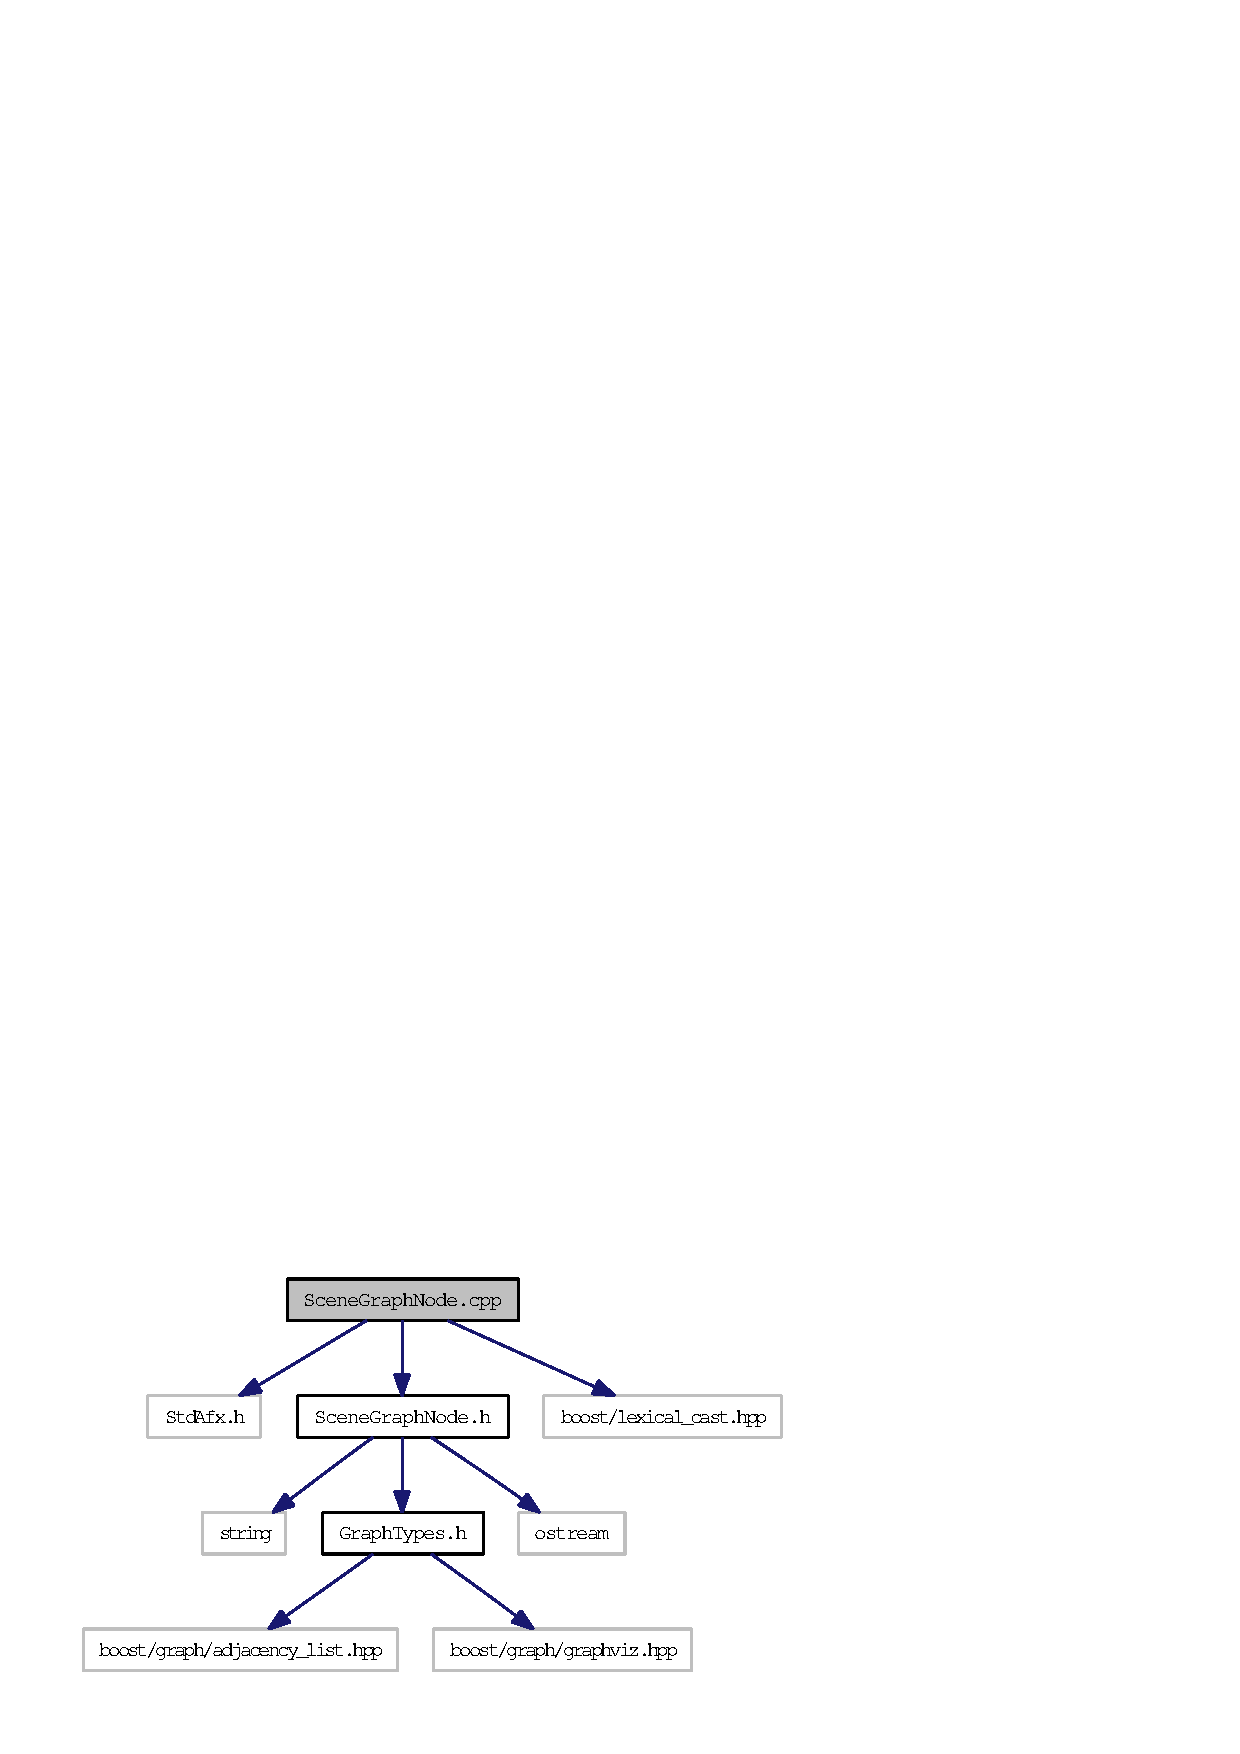
\includegraphics[width=189pt]{SceneGraphNode_8cpp__incl}
\end{center}
\end{figure}
\subsection*{Functions}
\begin{CompactItemize}
\item 
std::ostream \& {\bf operator$<$$<$} (std::ostream \&os, const {\bf SceneGraphNode} \&obj)
\end{CompactItemize}


\subsection{Function Documentation}
\index{SceneGraphNode.cpp@{SceneGraphNode.cpp}!operator$<$$<$@{operator$<$$<$}}
\index{operator$<$$<$@{operator$<$$<$}!SceneGraphNode.cpp@{SceneGraphNode.cpp}}
\subsubsection{\setlength{\rightskip}{0pt plus 5cm}std::ostream\& operator$<$$<$ (std::ostream \& {\em os}, const {\bf SceneGraphNode} \& {\em obj})}\label{SceneGraphNode_8cpp_afdd9566f57fdc8aa45f89687105c795}




Definition at line 61 of file SceneGraphNode.cpp.

References SceneGraphNode::toString().

Here is the call graph for this function:\nopagebreak
\begin{figure}[H]
\begin{center}
\leavevmode
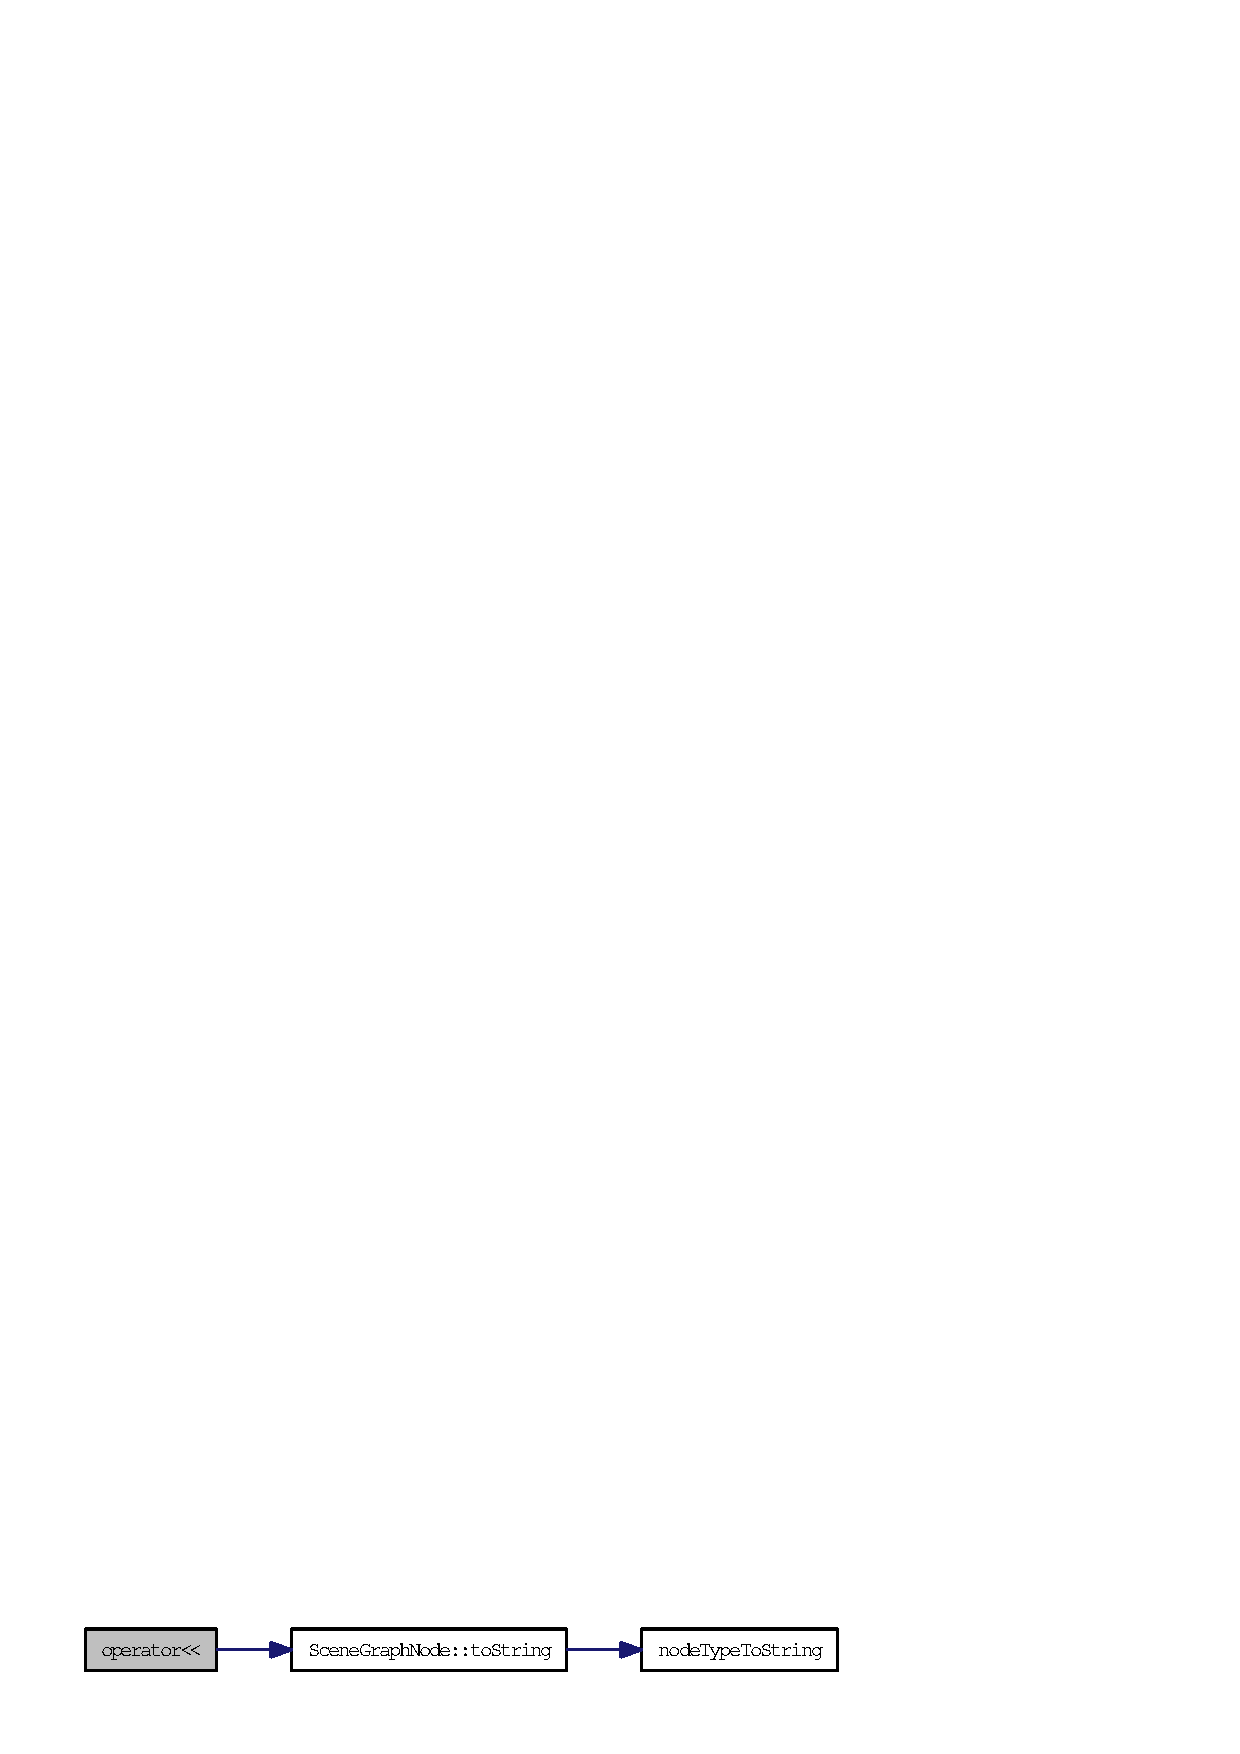
\includegraphics[width=203pt]{SceneGraphNode_8cpp_afdd9566f57fdc8aa45f89687105c795_cgraph}
\end{center}
\end{figure}
